% !TEX root=/home/tavant/these/manuscript/src/manuscript.tex


\section{Objectives of the chapter}
\label{sec-ch4objectiv}

In \Cref{sec-sheath_validation}, we have seen that the plasma-wall interaction observed in the \ac{2D} \ac{PIC} simulations were different from the models used.
We recall here the main observations of \cref{ch-2}.
We have conducted a parametric study on the wall emissivity by varying the crossover energy $\crover$ in the emission probability
\begin{equation*}
  \proba = \sigo + ( 1 - \sigo) \frac{\ek}{\crover},
\end{equation*} 
with $\ek$ the electron kinetic energy.
The \ac{SEE} rate (or yield) $\rate$ is the emission probability $\proba$ averaged over the electron flux at the wall.
With a Maxwellian flux of temperature $\Te$, we have 
\begin{equation}  \label{eq-rate2}
  \ratemaxw = \sigo + ( 1 - \sigo) \frac{2 \Te}{\crover}.
\end{equation}
The sheath model with \ac{SEE} predicts a potential drop between the sheath-edge and the wall of \citep{goebel2008,hobbs1967}
\begin{equation} \label{eq-dphi2}
  \dphi = \Te \log \lp [1 - \rate] \sqrt{\frac{m_i}{2 \pi m_e}}  \rp.
\end{equation}

\Cref{fig-Tevsproba2} shows both the plasma potential $\dphi$ and the \ac{SEE} rate $\rate$ measured in the \ac{PIC} simulations and obtained from the \cref{eq-rate2,eq-dphi2}.
We see that the plasma potential is overestimated for low values of $\rate$ by around 30\%.
Moreover, the \ac{SEE} rate is also overestimated.
 
\begin{figure}[hbt]
  \centering
  \begin{tabular}{@{} cc}
    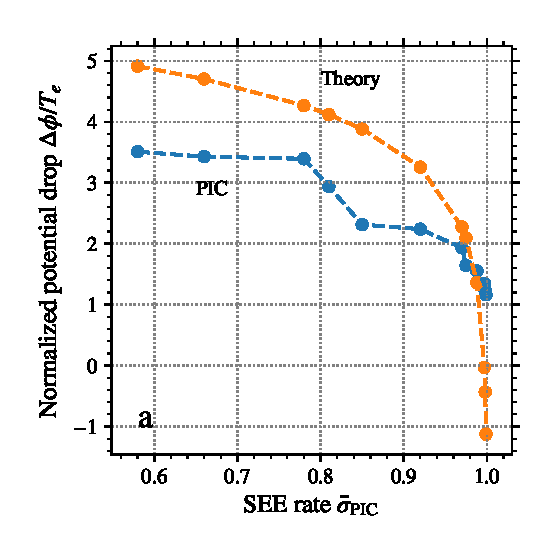
\includegraphics[width=0.45\textwidth]{phi_drop_6}
    &
    \subfigure{SEE_rates}{{\scriptsize b}}{20,18}
  \end{tabular}
  \caption{({\bf a}) Plasma potential drop to the wall $\dphi$ normalized by the electron bulk temperature $\Te$ as a function of the electron rate (blue) measured in the \acs{PIC} simulations and (orange) calculated with   \cref{eq-dphi2}; ({\bf b})  the \acs{SEE} rate $\rate$ (blue) measured in the PIC simulation, and (orange)  calculated with \cref{eq-rate2}}
  \label{fig-Tevsproba2}
\end{figure}

The discrepancy is most certainly due to the isothermal hypothesis.
In \cref{ch-3}, we have developed a sheath model that do not use the isothermal hypothesis, but instead the polytropic state law.
The objective of this chapter is to add to the polytropic sheath model of \cref{ch-3} the electron emission from the wall, in order to better predict the plasma-wall interaction.